\documentclass[11pt]{amsart}
\usepackage[margin=1in]{geometry}                % See geometry.pdf to learn the layout options. There are lots.
\geometry{letterpaper}                   % ... or a4paper or a5paper or ... 
%\geometry{landscape}                % Activate for for rotated page geometry
\usepackage[parfill]{parskip}    % Activate to begin paragraphs with an empty line rather than an indent
\usepackage{graphicx, enumerate}


\usepackage{subfig}
\usepackage[]{floatrow} 
\floatsetup[table]{style=plaintop}
\floatsetup[figure]{%style=BOXED, 
floatrowsep=qquad,   valign=c}
\floatsetup[subfigure]{subfloatrowsep=qquad, heightadjust=object, valign=c,  rowfill=yes}


\usepackage{amssymb}
\usepackage[normalem]{ulem}
\usepackage{epstopdf}
\DeclareGraphicsRule{.tif}{png}{.png}{`convert #1 `dirname #1`/`basename #1 .tif`.png}


\usepackage{tikz}
\usetikzlibrary{calc, through}
\usetikzlibrary{decorations.markings}
\usetikzlibrary{arrows}
\usetikzlibrary{positioning}

%\date{}                                           % Activate to display a given date or no date


\usepackage{hyperref}

\newcommand{\red}[1]{{\color{red}#1}}

%\newcommand{\deg}{\mathrm{deg}}

\newcommand{\bv}[1]{\ensuremath{\mathbf{#1}}}
\newcommand{\be}{\begin{enumerate}}
\newcommand{\ee}{\end{enumerate}}

\begin{document}
\begin{center}
\begin{Large} Math F307 \hfill Spring 2017

Homework Exercises 
\end{Large}
\end{center}
%\maketitle
%\section{}
%\subsection{}

\subsection*{Instructions for writing up homework}
\begin{itemize}
\item Although you are encouraged to work with your classmates on the homework assignments, you must write up the solutions individually.
\item Read the section!
 \item Use pen or non-smeary pencil. Do not have little scritchies on the side. 
 \item Staple your homework. 
 \item Write legibly, and leave lots of whitespace. Make sure your writing is dark enough to be readable. If this is problematic for you, consider typing your homework.
 \item Answer the question in complete sentences, where appropriate.
\item {\bf Write the \fbox{problem statements} as well as the answers. } This is not optional. \underline{Points will be deducted if you do not do this}.
\item Have headings indicating the section.
\item {\bf In the upper right hand corner of your top page,} write your name (first and last) on your assignment, along with the course number (Math 307) and which assignment it is.
\item {\bf You are expected to ask questions in class about the homework problems!}
\end{itemize}

\section*{Homework Set 10}

{\bf DUE Friday, April 7 \fbox{at the beginning of class}.} {\color{red} This is the day of your next exam!}



\subsection*{Planar graphs}


%\subsection*{Additional Problems}

To turn in:
\be
\item Find a plane drawing of the following graphs. Label your graph to demonstrate the isomorphism. For the left-hand graph, can you find a plane embedding with mirror symmetry?

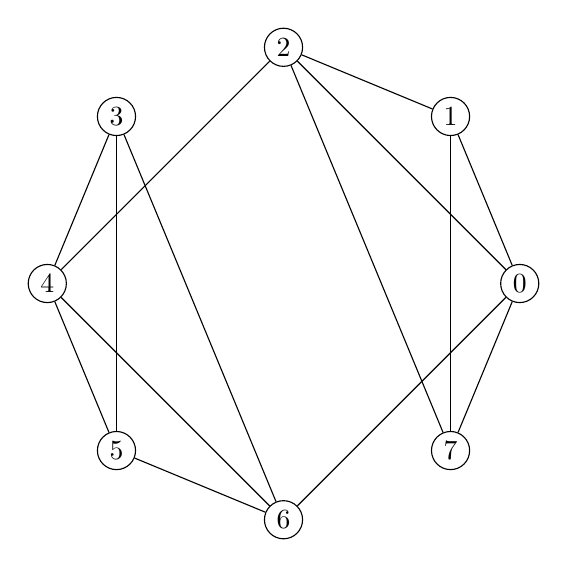
\begin{tikzpicture}
\foreach \i in {0, 1, ..., 7}{\node[draw, circle, inner sep = 2pt] (\i) at (360*\i/8: 3){\i};}
\foreach  \i/\j in {0/1, 0/2, 0/6, 0/7, 1/2, 1/7, 2/4, 2/7, 3/4, 3/5, 3/6, 4/5, 4/6, 5/6}
{\draw (\i) -- (\j);}
\end{tikzpicture}
\hspace{2cm}
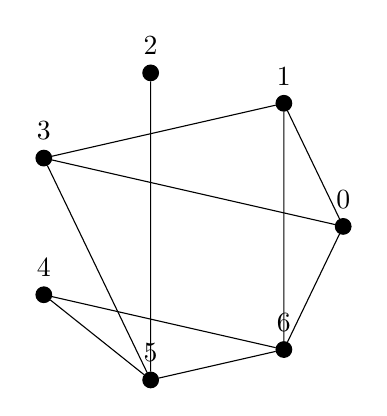
\begin{tikzpicture}[]
\foreach \i in {0, ...,6}{  \node[draw, circle, fill=black, inner sep = 2 pt, label={$\i$}](\i) at (\i*360/7: 2) {};}
\draw (1) -- (3)--(0);
\draw (2) -- (5) -- (4) -- (6) -- (0) --(1)--(6);
\draw (3) -- (5)--(6);
 \end{tikzpicture}

\item \be
\item Suppose that $G$ is a triangle-free, simple, \red{connected} plane graph \red{with at least 3 vertices}. Show that $E\leq 2V - 4$, by counting the edges around all the faces and using Euler's Theorem.

\item Use the previous result to show that $K_{3,3}$ is not planar.

\item Suppose that there are three houses on a road. Each house needs to be connected to gas, water, and electricity, via an underground connection. Is there a way to make all nine connections without any of the lines crossing each other? (Having to dig on one plane is much cheaper than having to route some of the connections below the others!) If not, what is the fewest number of crossings possible?
\ee

\item 
\be \item Suppose that $G$ is a connected simple plane graph, where every vertex is degree 3, that only has pentagons and hexagons as faces. Show that $G$ must have exactly 12 pentagons.
\item In the above situation, what is the smallest graph $G$ with this property? (Hint: what's the fewest number of hexagons possible in such a situation?)
\ee

\item Go find out about a planarity testing algorithm and describe how it works.





\ee


\end{document}